% BEGIN HEADER **************************************************************
\documentclass[usletter,11pt]{article}
\hyphenpenalty=5000

\usepackage[margin=1.40in]{geometry}
\usepackage{graphicx}
\usepackage{longtable}
\usepackage[table]{xcolor}
\usepackage{booktabs}
\usepackage{colortbl}
\usepackage{newcent}
\usepackage{sectsty}
\usepackage{fancyhdr}
\pagestyle{fancy}
\usepackage{calc}
\usepackage{listings}
\usepackage{array}
\usepackage{tikz}
\usepackage{amsmath}
\renewcommand{\headrule}{{\color{brightOrange}%
  \hrule width\headwidth height\headrulewidth \vskip-\headrulewidth}}
\renewcommand{\footrule}{{\color{brightOrange}%
  \hrule width\headwidth height\headrulewidth \vskip-\headrulewidth}}

\newcommand{\referee}[1]{
\begin{center}
\begin{tikzpicture}
\node[fill=paleOrange, rounded corners=0.3cm]{
 \parbox{\textwidth}{
  \vspace{0.15cm}
#1
  \vspace{0.15cm}
 }
};
\end{tikzpicture}
\end{center}
}

\newcommand{\member}[2]
{ \noindent
{ \color{softBlue}  #1 - } #2
\vspace{0.2cm}
}

\fancyheadoffset[LE,RO]{\marginparwidth}
\fancyfootoffset[LE,RO]{\marginparwidth}
\fancyhead{} % clear all header fields
\fancyhead[LE,RO]{\color{softBlue}  \sffamily The Data Exchange File Format}

\fancyfoot{} % clear all header fields
\fancyfoot[L]{\vspace{0.1cm}
\includegraphics[width=0.35\textwidth]{figures/dx_logo_header.pdf}}
\fancyfoot[R]{\vspace{1.0cm}\color{softBlue}\thepage}

\usepackage{setspace}

\definecolor{tableBlue}{RGB}{231,244,249}
\definecolor{linkBlue}{RGB}{32,75,165}
\definecolor{brightOrange}{RGB}{210,131,37}
\definecolor{ironGrey}{RGB}{64,73,78}
\definecolor{steelGrey}{RGB}{70,91,102}
\definecolor{cloudyGrey}{RGB}{104,132,150}
\definecolor{lightGrey}{RGB}{184,198,206}
\definecolor{softBlue}{RGB}{29,97,134}
\definecolor{paleOrange2}{RGB}{233,185,128}
\definecolor{paleOrange}{RGB}{248,219,167}
\definecolor{typeGreen}{RGB}{19,101,106}

\usepackage{caption}
\DeclareCaptionFont{white}{\color{white}}
\DeclareCaptionFont{softBlue}{\color{softBlue}}
\DeclareCaptionFormat{listing}{\colorbox{softBlue}{\parbox{\textwidth}{\hspace{15pt}#1#2#3}}}
\captionsetup[lstlisting]{format=listing,labelfont=white,textfont=white,
  singlelinecheck=false, margin=0pt, font={sf,footnotesize}}
\captionsetup[figure]{labelfont={softBlue,bf},
 singlelinecheck=false, margin=0pt, font={small}}
\captionsetup[table]{labelfont={softBlue,bf},
 singlelinecheck=false, margin=0pt, font={footnotesize},justification=centering}



\newcommand{\HRule}{{\color{brightOrange} \rule{\linewidth}{0.5mm}}}

\allsectionsfont{\color{softBlue} \usefont{OT1}{pag}{b}{n}\selectfont}

\usepackage[linkcolor=softBlue,colorlinks=true,urlcolor=softBlue]{hyperref}

\setcounter{secnumdepth}{6}
\setcounter{tocdepth}{6}

% END HEADER ****************************************************************

% BEGIN MAIN DOCUMENT *******************************************************
\begin{document}
\pagestyle{empty}

% BEGIN TITLE PAGE **********************************************************
\begin{center}
\vspace*{2.5cm}

\HRule \\[0.6cm]
\begin{spacing}{2.0}

{\color{softBlue} \Huge \sffamily The Scientific Data Exchange}\\[0.15cm]
{\color{softBlue} \Huge \sffamily Introductory Guide}\\[0.15cm]
\end{spacing}
\HRule \\[1.0cm]
{\Large \color{softBlue} \sffamily \url{http://www.aps.anl.gov/DataExchange}}\\[1.0cm]
{\Large \color{softBlue} \sffamily Version 0.9.5}\\[1.0cm]
{\Large \color{softBlue} \sffamily \today}

\end{center}
\newpage
% END TITLE PAGE ************************************************************

%****************************************************************************

\begin{longtable}{p{1.2cm} p{2.6cm}  p{9.9cm}}
\caption{Version history} \\
\bfseries Version & \bfseries Date & \bfseries Notes \\ 
\endhead
\toprule
0.8.9 & Feb. 25, 2012 & de carlo: first document draft. \\
0.9.0 & May 25, 2012 & saunders: Extensive reworking of document structure and some definitions. \\
0.9.1 & April 20, 2013 & de carlo: added Python examples and corrected minor tomography definitions. Changed provenance definition.\\
0.9.2 & June 27, 2013 & de carlo: added sample\_x and sample\_y in the raw data exchange definition to store sample projection position at each point during data collection. Modified Python example 5.\\
0.9.3 & Nov 8, 2013 & vine: Added CDI section. Added Python examples.\\
\bottomrule
\label{table:SI}
\end{longtable}

%****************************************************************************
\newpage

\pagestyle{fancy}
\pagenumbering{Roman}

% TOC ***********************************************************************
\tableofcontents
% ***************************************************************************

\newpage

\pagenumbering{arabic}
\setcounter{page}{1}

%****************************************************************************
\section{Introduction}

This document is a guide to the basic design principles and core guidelines
for the Data Exchange file format. Briefly, Data Exchange is a set of
guidelines for storing scientific data and metadata in a Hierarchical Data
Format 5 (HDF5) file (\url{http://www.hdfgroup.org/HDF5}). The design
guidelines for Data Exchange provide a starting point to which one
may add custom data and metadata to solve particular problems. 

HDF5 has many important characteristics for scientific data storage.
It offers platform-independent binary data storage with optional compression, 
hierarchical data ordering, and support for MPI-based parallel computing.
Data are stored with alphanumeric tags, so that one can examine a 
HDF5 file's contents with no knowledge of how the file writing program 
was coded. Tools for this examination include the 
HDF5-supplied command-line utility 
\href{http://www.hdfgroup.org/HDF5/doc/RM/Tools.html#Tools-Dump}{\texttt{h5dump}} 
to examine the contents of any HDF5 file, or the freely-available Java program 
\href{http://www.hdfgroup.org/hdf-java-html/hdfview/}{\texttt{HDFView}} to interactively examine the file.

Why not just use the \href{http://www.nexusformat.org/}{NeXus} format? While we employ some of the naming conventions of NeXus, the format has not been as widely adopted in the synchrotron radiation community as it has in the neutron beam research community.  NeXus is normally based on use of an Application Programming Interface (API) for all file access; this API has not in the past had well-debugged versions available for all platforms and languages.  NeXus has not supported recent HDF5 extensions such as dimension scales, and it has not had definitions for tracking the provenance of subsequent analysis steps.  "Straight" HDF5 calls can make use of the HDF5 group's support of a wide variety of computer platforms, and built-in support in MATLAB, IDL, and Python; it also has support for MPI-based parallel access to files.  As a result, we have sought to follow many naming conventions from NeXus, but to aim for a more streamlined file structure with necessary definitions added.

This reference guide describes the basic design principles of Dat Exchange, examples of their
application, a core reference for guidelines common to most uses, and coding
examples.

%****************************************************************************

\section{The Design of Data Exchange} 

For various reasons, many x-ray techniques developed at synchrotron facilities
around the world are unable to directly compare results due to their 
inability to exchange data and software tools. The aim of Data Exchange is to
define a simple file format offering few basic rules and allowing each
community to extend and add technique specific components. The goal is to
provide extensibility in defining data, meta data and
provenance information in a simple way that can be easily adopted by various
x-ray techniques.

The Data Exchange format is implemented using Hierarchical Data Format 5
(HDF5), which offers platform-independent binary data storage with optional
compression, hierarchical data ordering, and self-describing tags so that one
can examine a HDF5 file's contents with no knowledge of how the file writing
program was coded.

The aim and the scope of Data Exchange is very similar to the Coherent X-ray
Imaging  Data Bank file format (CXI), so whenever possible we will use the
same conventions, name tags, and reference system. This document is using a
similar diagram definition set by Filipe R. N. C. Maia in "CXI file format"
(\url{http://cxidb.org/cxi.html}), with a few minor modifications for Data
Exchange definitions.

The core principle of Data Exchange is that it must be simple enough that it
is not necessary to use a support library beyond core HDF5. The simplicity of
Data Exchange makes it easy for anyone to either look at an example file 
using h5dump or HDFView, or to look at example code in language X, and 
then create their own read and write routines in language Y.

The simplest Data Exchange file provides information
sufficient to share a multidimensional data array. In
this simplest form, Data Exchange implements only one "exchange"
group. The "exchange" definition is designed to allow for simple exchange of
images, spectra, and other forms of beamline detector data with a minimum of
fields. This definition is essentially a technique-agnostic format for
exchanging data with others. Data Exchange is also designed to be extended
to include technique-specific data and metadata.  This is
achieved by providing optional, but clearly defined, metadata components to
the base definition.

\subsection{HDF5}

The HDF5 format is the basis of the Data Exchange format. Data Exchange, like
CXI, is not a completely new file format, but simply a set of rules designed
to create HDF5 files with a common structure to allow a uniform and
consistent interpretation of such files.

HDF5 was chosen as the basis because it is a widely used high performance
scientific data format which many programs can already, at least partially,
read and write. It also brings with it the almost automatic fulfillment of the
Data Exchange requirements, i.e. simplicity, flexibility and extensibility.
HDF5 version 1.8 or higher is required as previous versions don't support all
features required by Data Exchange.

\subsection{Data types}

Data Exchange uses the same CXI convention for data types as defined at 
\url{http://cxidb.org/cxi.html} using HDF5 native datatypes.  The data should
be saved in the same format as it was created/acquired. For example CCD images
acquired as 16 bit integers should be saved using the {\tt H5T\_NATIVE\_SHORT}
HDF5 type. In this way all cross platform big-little endian issues reading and
writing files are eliminated.

\subsection{Root Level Structure}
\label{DataExchange}

While HDF5 gives great flexibility in data storage, straightforward file
readability and exchange requires adhering to an agreed-upon naming and
organizational convention. To achieve this goal, Data Exchange adopts a
layered approach by defining a set of \emph{mandatory} and
{\tt optional} fields. 

The general structure of a Data Exchange file is shown in table~\ref{tab:genrules}.
The most basic file must have an "implements" string, and an "exchange" group at
the root level/group of the HDF5 file. Optional "measurement" and "provenance"
groups are also defined. Beyond this, additional groups may be added to meet
individual needs, with guidelines suggesting the best structure.

\begin{table}[h!]\sffamily
\centering
\footnotesize
\caption{Data Exchange Top Level Members}
\label{tab:genrules}
\rowcolors{1}{white}{tableBlue}
\begin{tabular}{l l l}
\toprule
\bfseries Member     & \bfseries Type & \bfseries Example \\
\midrule

\emph{implements} & string dataset & "exchange:measurement:provenance" \\
\hyperref[sec:exchange]{\emph{exchange}} &  group  & \\
\hyperref[table:measurement]{\tt{measurement}} &  group  & \\
\hyperref[table:provenance]{\tt{provenance}} & group & \\
\bottomrule
\end{tabular}
\end{table}

\begin{description}
\item[\emph{implements}] \hfill \\
{Mandatory scalar string dataset in the root of the HDF5 file whose
value is a colon separated list that shows which components are present in the
file. All components listed in the \emph{implements} string are to be groups
placed in the HDF5 file at the root level/group. In a minimal Data
Exchange file, the only mandatory item in this list is \emph{exchange}. A more
general Data Exchange file also contain {\tt{measurement}} and possibly  
{\tt{provenance}}, in which case the implements string would be:
"\emph{exchange}: {\tt{measurement}}: {\tt{provenance}}"}

\item[\emph{exchange}] \hfill \\
{Mandatory group containing one or more arrays that
represent the most basic version of the data, such as raw or normalized
optical density maps or a elemental signal map.  \emph{Exchange\_$N$} is
used when more than one core dataset or derived datasets are saved in the file.
The \emph{exchange} implementation for specific techniques are defined
in separate sections in the Reference Guide.}

\item[\tt measurement] \hfill \\
{Optional group containing the measurement made on the
sample.  {\tt Measurement} contains information about the {\tt sample}  and
the  {\tt instrument}. {\tt Measurement\_$N$} is used when more than one
measurement is stored in the same file.}

\item[\tt provenance] \hfill \\
{Optional group containing information about the status
of each processing step.}

\end{description}

In a  Data Exchange file, each dataset has a unit defined using the
{\tt units} attribute. {\tt units}  is not mandatory - if omitted, the default
unit as defined in Appendix~\ref{appendix:units} is used.

The detailed rules about how to store datasets within the exchange group
are best shown through examples in the next section. Detailed reference information
can be found in the \hyperref[sec:corereference]{Data Exchange Core Reference} section.


%****************************************************************************

\newpage

%****************************************************************************

\section{Data Exchange by Example}
The examples in this section show how one can store data for imaging experiments using the Data 
Exchange format. It is general enough, however, to show how Data Exchange can be extended or adapted 
to other techniques. These examples are meant to give a flavor for our approach. A complete reference to 
the core structure can be found in Section \ref{sec:corereference}. Technique specific extensions to the core 
structure can be found at the end of the Reference Guide.

\subsection{Diagram color code}
All the diagrams in this section follow the color conventions shown in Figure \ref{fig:DiagramColorCode}. 
The basic elements are HDF5 datasets, attributes, and groups. We also support internal references to 
elements in the file by a simple scalar string that holds the path of the dataset within the file. On the 
diagram, this is shown as a reference dataset that points to the referred-to dataset. Note that we use this 
mechanism rather than HDF5 hard or soft links
\label{DiagramColorCode}

\begin{figure}[h!]
\centering
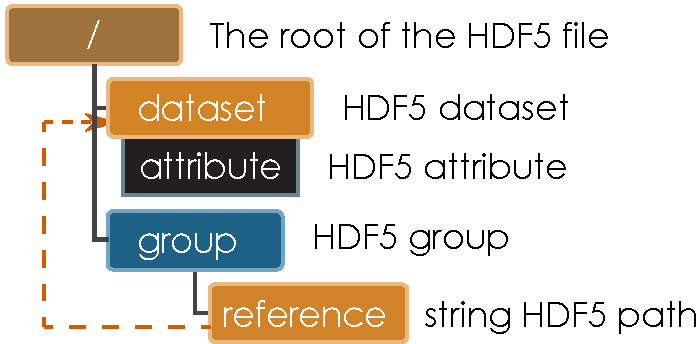
\includegraphics[width=0.5\textwidth]{figures/dx_DiagramColorCode.pdf}
\caption{Explanation of the color code used in the diagrams}
\label{fig:DiagramColorCode}
\end{figure}

\subsection{A minimal Data Exchange file for imaging}
Figures \ref{fig:Minimal1} shows a diagram of a minimal Data Exchange file to store a single projection 
image.  It is strongly encouraged that all datasets shall have a units attribute. The axes of the dataset are 
not specified in this minimal
case, and can be assumed to be x and y with a zero-based integer sequence, or more simply, pixels.
 
\begin{figure}[h!]
\centering
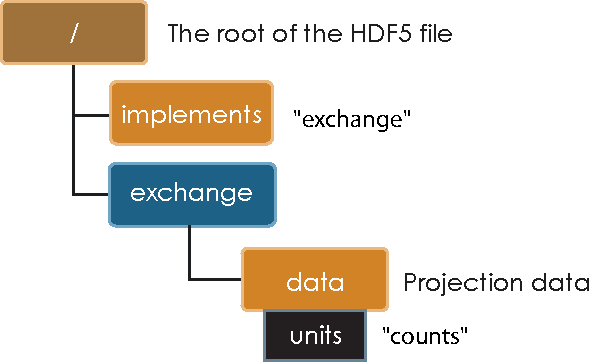
\includegraphics[width=0.5\textwidth]{figures/dx_Minimal1.pdf}
\caption{Diagram of a minimal Data Exchange file for a single image.}
\label{fig:Minimal1}
\end{figure}

\subsection{Storing and describing a multidimensional dataset}
A multidimensional dataset should be described as fully as possible, with units for the dataset as well as 
dimension descriptors (that also have units defined). There are also additional descriptive fields available 
such as title and description. The order of dimensions in the dataset should put the slowest changing 
dimension first, and the fastest changing dimension last. 

It is strongly encouraged that all datasets have a units attribute. The string value for units should preferably 
be an SI unit, however well understood non-SI units are acceptable, in particular "degrees". The units 
strings should conform to those defined by UDUNITS at {http://www.unidata.ucar.edu/software/udunits}. 
While UDUNITS is a software package, it contains simple XML files that describe units strings and 
acceptable aliases.

The axes of a multidimensional dataset are described through the use of additional one-dimensional 
datasets (dimension descriptors), one for each axis in the main dataset. Take for example a 3-dimensional 
cube of images, with axes of x, y, and z where z represents the angle of the sample when each image was 
taken. There should be 3 additional one-dimensional datasets called x, y, and z where x and y contain an 
integer sequence, and z contains a list of angles. X and y have units of "counts" and z has units of 
"degrees". To simplify, it is acceptable to omit x and y, since the default interpretation will always be an 
integer sequence. 

The dimension descriptors (x, y, and z) can be associated with the main dataset through two mechanisms. 
The HDF5 libraries contain a function call H5DSattach\_scale to "attach" a dimension descriptor 
dataset to a given dimension of 
the main dataset. HDF5 takes care of entering several attributes in the file that serve to keep track of this 
association. If the particular programming language you work in does not support this HDF5 function, then 
you can instead add a string attribute to your main dataset called axes. The axes attribute is simply a colon 
separated string naming the dimension descriptor datasets in order, so "z:y:x" in this case. Additional 
examples below show this in action.

\subsection{Storing projections, dark fields, and white fields}
\label{section:minimalTomo}

A tomographic data set consists of a series of projections, dark and white field images. The dark and white fields must have the same projection image dimensions and can be collected at any time before, after or during the projection data collection. The angular position of the tomographic rotation axis, theta, can be used to keep track of when the dark and white images are collected.  These examples show projection, dark, and white images saved in three 3D arrays as shown in Figure \ref{fig:MinimalTomo0} and \ref{fig:MinimalTomo1} using, by default, the natural HDF5 order of the a multidimensional array (rotation axis, ccd y, ccd x), i.e. with the fastest changing dimension being the last dimension, and the slowest changing dimension being the first dimension. If using the default dimension order, the axes attribute "theta:y:x" can be omitted. The {\tt{axes}} attribute is mandatory if the 3D arrays use a different axes order. This could be the case when, for example, the arrays are optimized for sinogram read ({\tt{axes}} = "y:theta:x"). As no units are specified the data is assumed to be in ``counts'' with the axes (x, y) in pixels. 

If the positions of the rotation axis for each projection, dark, and white images are not specified via theta dimension scale datasets, it is assumed that the raw projections are taken at equally spaced angular intervals between 0 and 180 degree, with white and dark field collected at the same time before or after the projection data collection.

\begin{figure}[h!]
\centering
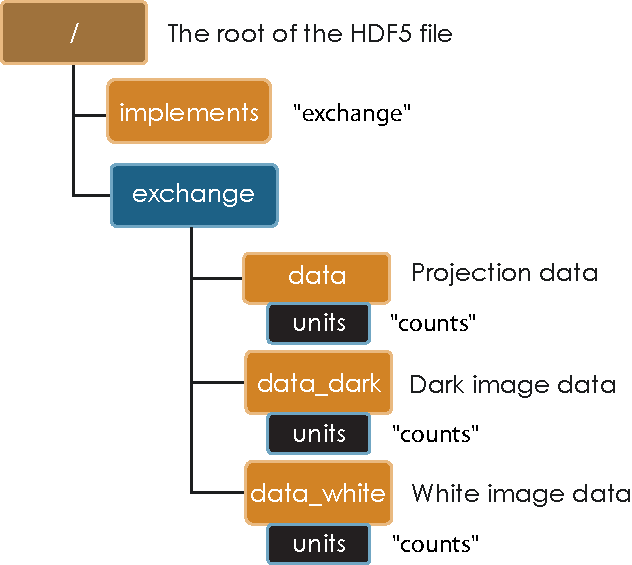
\includegraphics[width=0.5\textwidth]{figures/dx_MinimalTomo0.pdf}
\caption{Diagram of a minimal Data Exchange file for a single tomographic data set including raw projections, dark, and white fields.}
\label{fig:MinimalTomo0}
\end{figure}

\begin{figure}[h!]
\centering
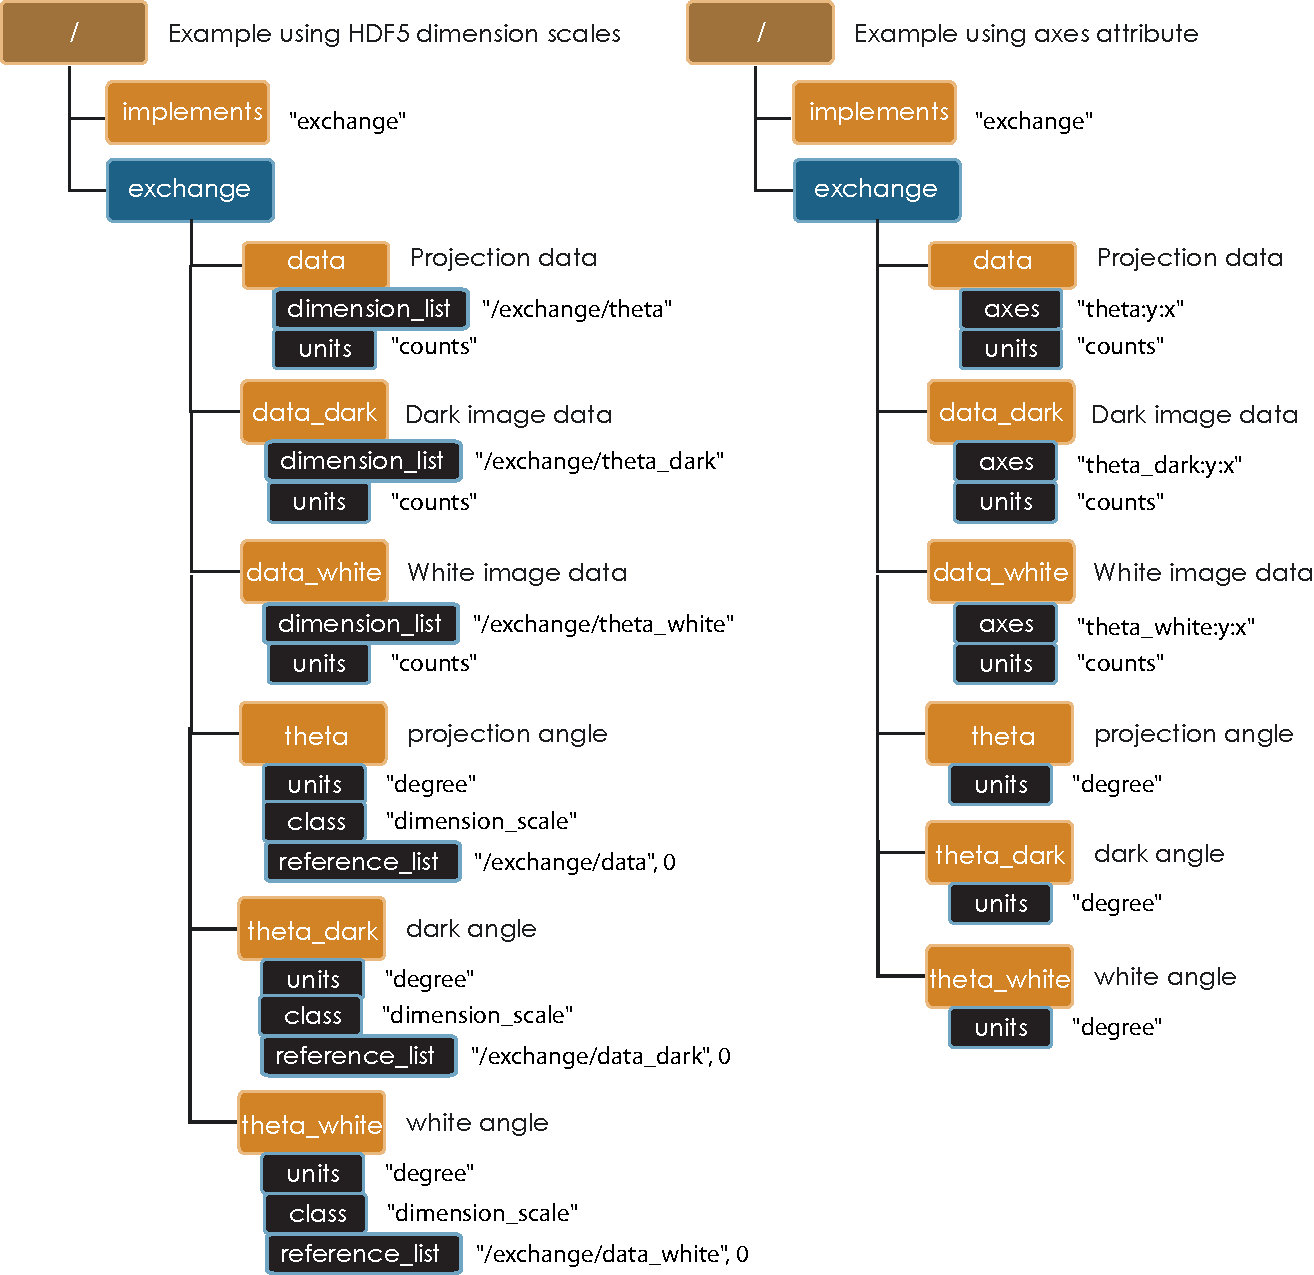
\includegraphics[width=0.8\textwidth]{figures/dx_MinimalTomo1.pdf}
\caption{Diagram of a single tomographic data set including raw 
projections, dark and white fields. In this case, there are additional dimension descriptor
datasets theta, theta\_dark, and theta\_white that contain the positions of the rotation axis
for each projection, dark, and white image. The lefthand example shows this as it would
appear using the HDF5 H5DSattach\_scale function. The righthand example shows this as it would
appear by manually adding an axes attribute (for cases where H5DSattach\_scale is unavailable).}


\label{fig:MinimalTomo1}
\end{figure}

\subsection{A typical Data Exchange file for tomography}
A series of tomographic data sets are typically collected changing the instrument status (energy, detector or 
optics position) or changing the sample status (position, environment etc.). Figure \ref{fig:MinimalTomo2}, 
\ref{fig:MinimalTomo3} and \ref{fig:MinimalTomo4}  show the content of files changing the sample 
temperature, the x-ray source energy and detector-sample distance. 

\subsubsection{Sample Temperature Scan}
\begin{figure}[h!]
\centering
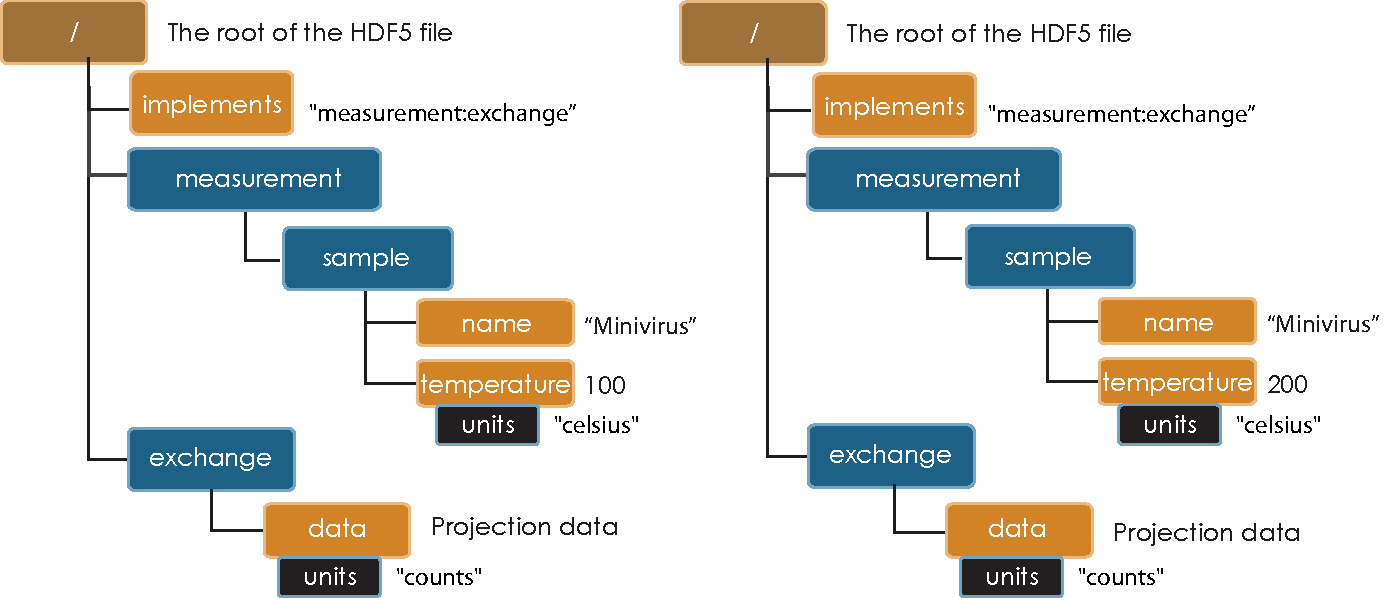
\includegraphics[width=1.0\textwidth]{figures/dx_MinimalTomo2.pdf}
\caption{Diagram of two tomographic data sets taken at two different sample temperatures (100 and 200 celsius).}
\label{fig:MinimalTomo2}
\end{figure}

\clearpage
\subsubsection{X-ray Energy Scan}
\begin{figure}[h!]
\centering
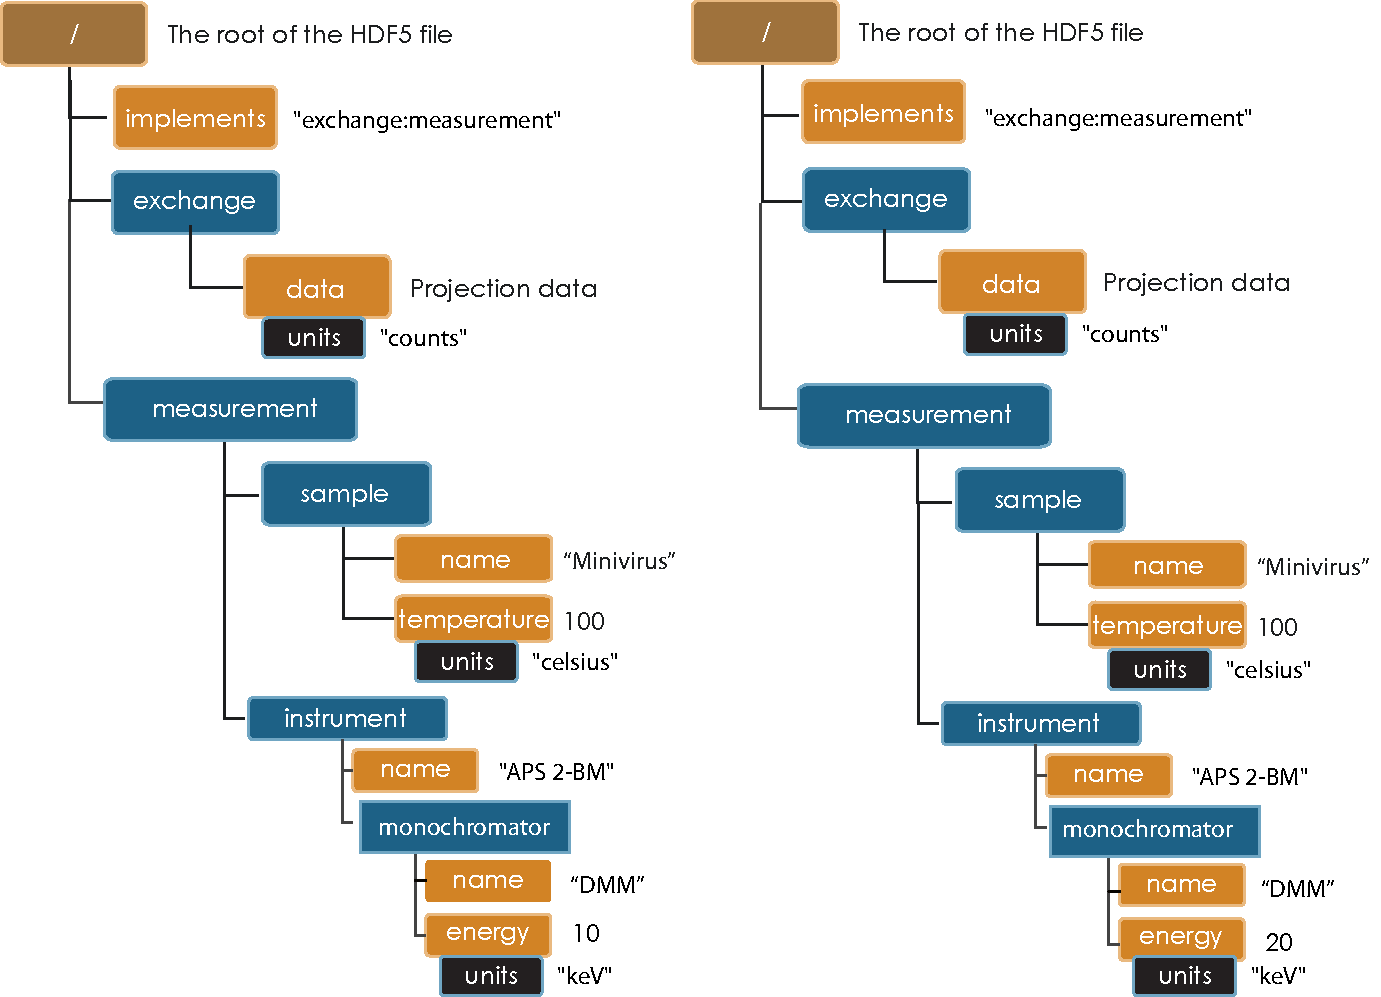
\includegraphics[width=0.8\textwidth]{figures/dx_MinimalTomo3.pdf}
\caption{Diagram of two tomographic data sets taken at two different energy (10 and 20 keV).}
\label{fig:MinimalTomo3}
\end{figure}

\clearpage
\subsubsection{Detector-sample Distance Scan}
\begin{figure}[h!]
\centering
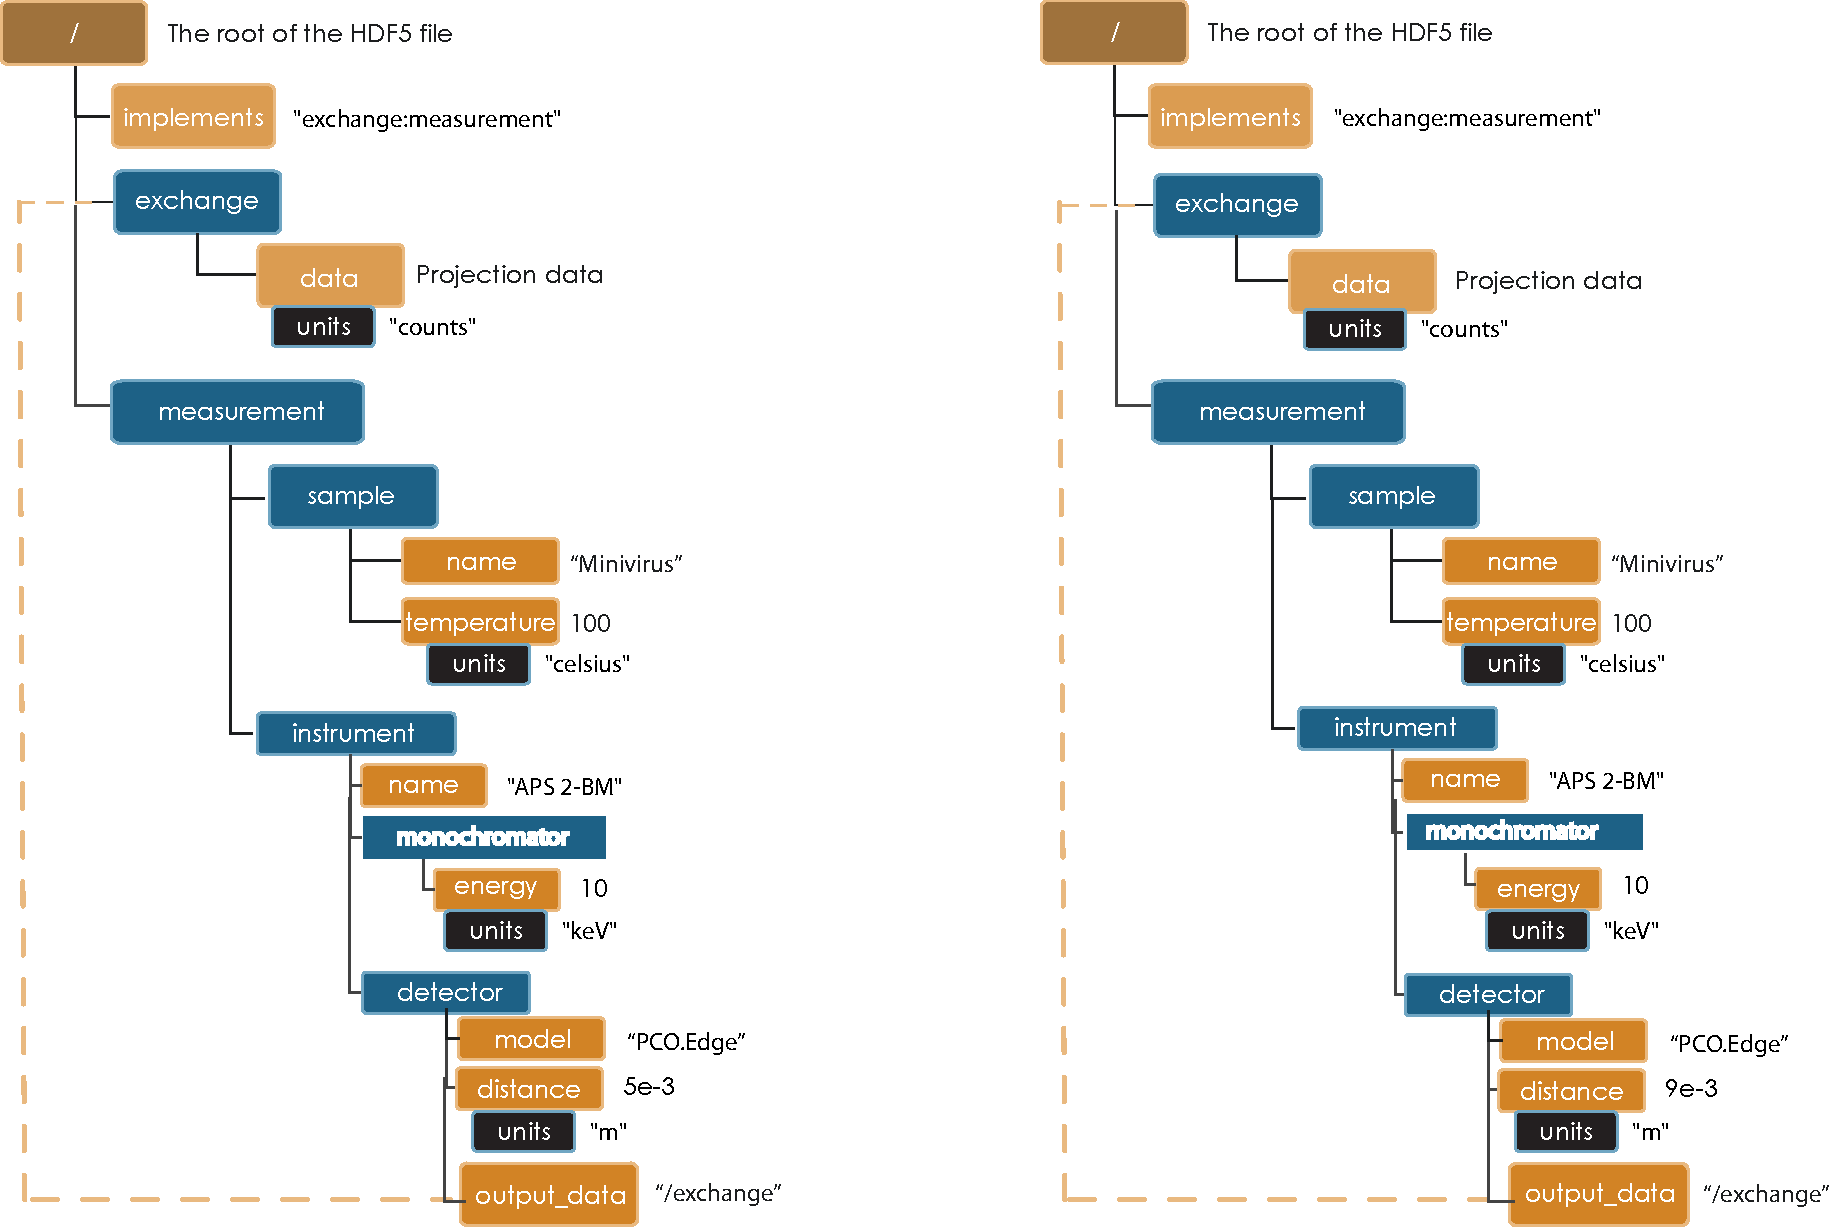
\includegraphics[width=0.8\textwidth]{figures/dx_MinimalTomo4.pdf}
\caption{Diagram of two tomographic data sets collected with two different detector-sample distances (5 and 9 mm). Note the use of {\tt output\_data} dataset to associate the detector with the exchange group generated from the acquisition.}
\label{fig:MinimalTomo4}
\end{figure}

\subsubsection{Series of Tomographic Measurements}

A series of tomographic measurements, when relevant, can be stored in the same file appending \_$N$ to the measurement tag. In nano tomography experiments, for example, the detector field of view is often smaller than the sample. To collect a complete tomographic data set, it is necessary to raster the sample across the field of view moving its x and y location. Figure \ref{fig:NanoTomo1}  shows a file from a nano tomography experiment when the sample rasters through the field of view.  

There are limits to this approach, as one clearly does not want to have hundreds of measurement groups in a file (or multiple files) where most of the metadata is the same. For measurements where there are many "positioner" values (aka a "scan"), it is more sensible to add dimension(s) to the exchange dataset, and describe the "positioner" values as dimension scales. This is a judgement left to the user.

\begin{figure}[h!]
\centering
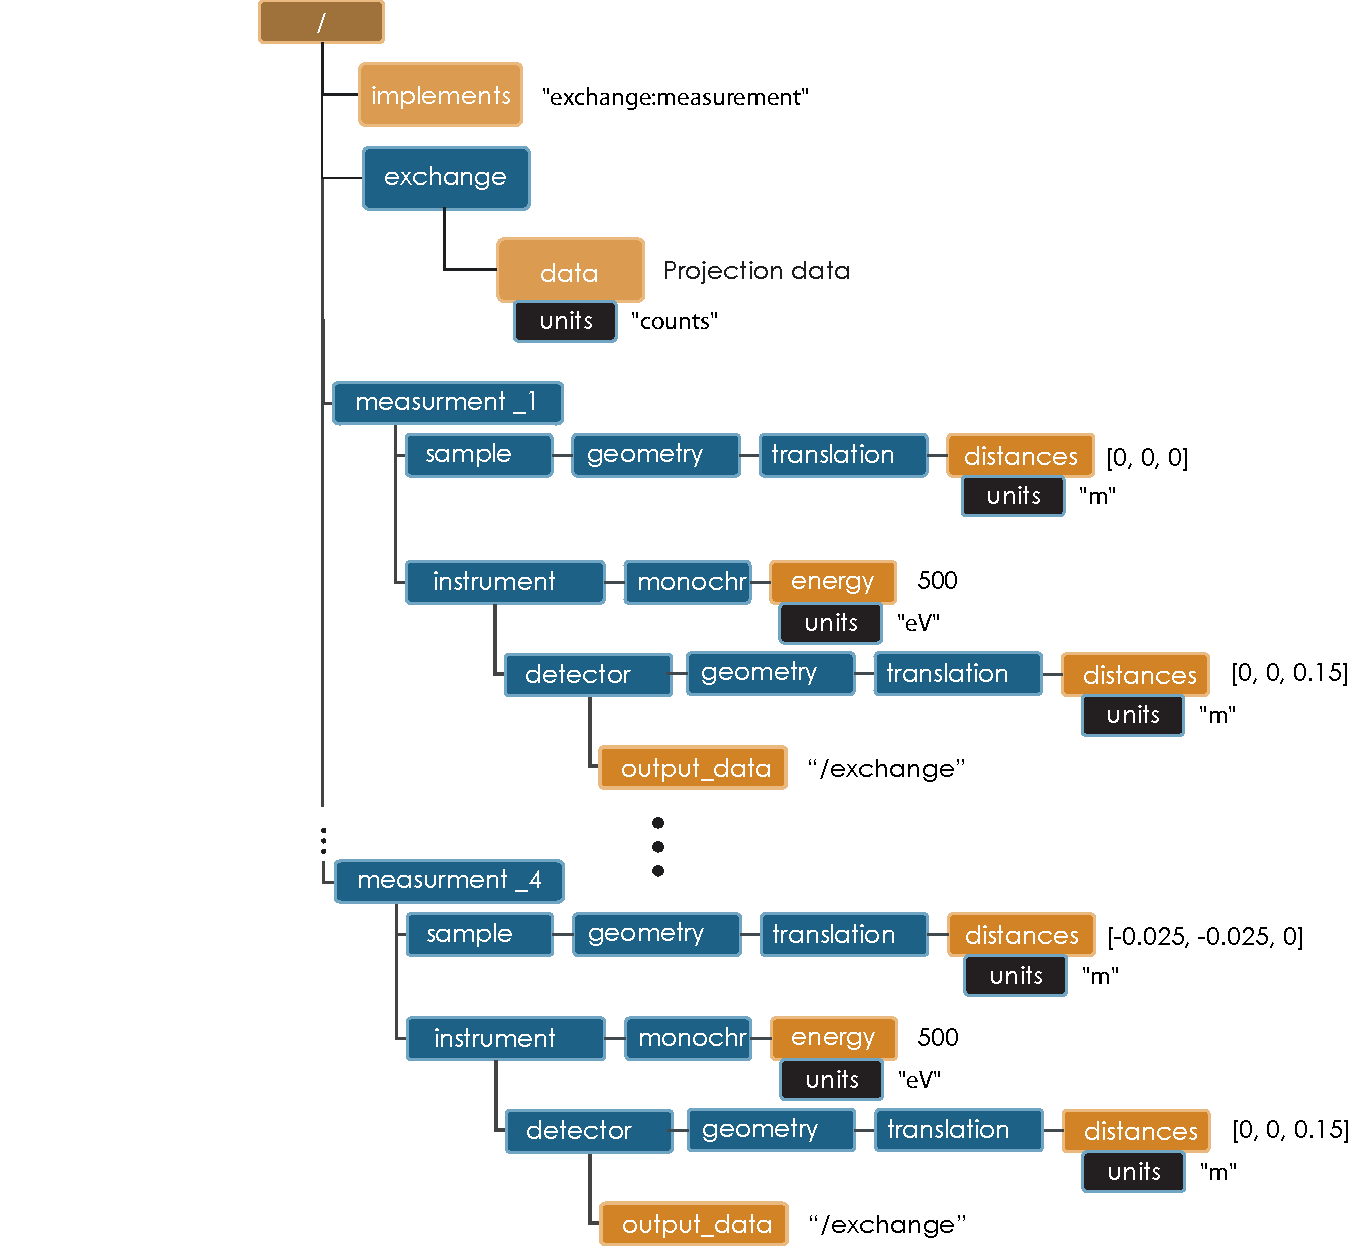
\includegraphics[width=0.9\textwidth]{figures/dx_NanoTomo1.pdf}
\caption{Diagram of a file with 4 tomographic data sets from a nano tomography experiment.}
\label{fig:NanoTomo1}
\end{figure}

%****************************************************************************

\newpage

%****************************************************************************

\section{Data Exchange Core Reference}
\label{sec:corereference}

%****************************************************************************
\subsection{Top level (root)}
\label{table:top}

This node represents the top level of the HDF5 file and holds some general 
information about the file.

\begin{table}[h!]\sffamily
\centering
\footnotesize
\caption{Top Level Members}
\rowcolors{1}{white}{tableBlue}
\begin{tabular}{l l l}
\toprule
\bfseries Member & \bfseries Type & \bfseries Example \\
\midrule

\emph{implements} & string dataset & "exchange:measurement:provenance" \\
\hyperref[exchange:tomography]{\emph{exchange\_$N$}} & group & \\
\hyperref[table:measurement]{\tt{measurement\_$N$}} & group & \\
\hyperref[table:provenance]{\tt{provenance}} & group & \\

\bottomrule
\end{tabular}
\end{table}

\begin{description}
\item[\emph{implements}] \hfill \\
{A colon separated list that shows which components are present in the file. The
only \emph{mandatory} component is \emph{exchange}. A more general Data Exchange
file also contains {\tt measurement} and {\tt provenance} information, if so 
these will be declared in implements as "exchange:measurement:provenance"}

\item[\emph{exchange\_$N$}] \hfill \\
{The data taken from measurements or processing. Dimension descriptors within the group may also serve to describe "positioner" values involved in a scan. }

\item[\tt{measurement\_$N$}] \hfill \\
{Description of the sample and instrument as configured for the measurement. This group is appropriate for relatively static metadata.  For measurements where there are many "positioner" values (aka a "scan"), it is more sensible to add dimension(s) to the exchange dataset, and describe the "positioner" values as dimension scales rather than record the data via multiple matching measurement\_N and exchange\_N groups. This is a judgement left to the user.}

\item[\tt{provenance}] \hfill \\
{The Provenance group describes all process steps that have been applied to the
data.}
\end{description}

\clearpage

%****************************************************************************
\subsection{Exchange}
\label {sec:exchange}
The exchange group is where scientific datasets reside. This group
contains one or more array datasets containing n-dimensional data and optional 
descriptions of the axes (dimension scale datasets). Exactly how this group is
used is dependent on the application, however the general idea is that
one exchange group contains one cohesive dataset. If, for example, the
dataset is processed into some other form, then another exchange group is
used to store the derived data.

Multiple exchange groups are numbered consecutively as exchange\_$N$. At a 
minimum, each exchange group should have a primary dataset named
data. The title is optional.

\begin{table}[h!]\sffamily \footnotesize
\centering
\caption{Exchange Group Members}
\rowcolors{1}{white}{tableBlue}
\begin{tabular}{l l l}
\toprule
\bfseries Member     & \bfseries Type & \bfseries Example \\
\midrule
\tt{title}  & string dataset & "tomography projections" \\
\hyperref[data:attr]{\emph{data}}  &  array dataset & {n-dimensional dataset} \\
\bottomrule
\end{tabular}
\end{table}

\begin{description}
\item[\tt{title}] \hfill \\
{Descriptive title for data dataset.}

\item[\emph{data}] \hfill \\
{The primary scientific dataset. Additional related datasets may have any
arbitrary name. Each dataset should have a units and description attribute.
Discussion of dimension descriptors and optional axes attribute is covered
in Section \ref{sec:multidims}.}
\end{description}

\begin{table}[h!]\sffamily \footnotesize
\centering
\caption{data attributes}
\label{data:attr}
\rowcolors{1}{white}{tableBlue}
\begin{tabular}{l l l}
\toprule
\bfseries Attribute     & \bfseries Type & \bfseries Example \\
\midrule
\tt{description}  & string attribute & "transmission"  \\
\tt{units}  & string attribute & "counts"  \\
\bottomrule
\end{tabular}
\end{table}

\subsubsection{Storing and describing a multidimensional dataset}
\label{sec:multidims}
A multidimensional dataset should be described as fully as possible, with units for the dataset as well as 
dimension descriptors (that also have units defined). There are also additional descriptive fields available 
such as title and description. The order of dimensions in the dataset should put the slowest changing 
dimension first, and the fastest changing dimension last. 

It is strongly encouraged that all datasets have a units attribute. The string value for units should preferably 
be an SI unit, however well understood non-SI units are acceptable, in particular "degrees". The units 
strings should conform to those defined by UDUNITS at {http://www.unidata.ucar.edu/software/udunits}. 
While UDUNITS is a software package, it contains simple XML files that describe units strings and 
acceptable aliases.

The axes of a multidimensional dataset are described through the use of additional one-dimensional 
datasets (dimension descriptors), one for each axis in the main dataset. Take for example a 3-dimensional 
cube of images, with axes of x, y, and z where z represents the angle of the sample when each image was 
taken. There should be 3 additional one-dimensional datasets called x, y, and z where x and y contain an 
integer sequence, and z contains a list of angles. X and y have units of "counts" and z has units of 
"degrees". To simplify, it is acceptable to omit x and y, since the default interpretation will always be an 
integer sequence. 

The dimension descriptors (x, y, and z) can be associated with the main dataset through two mechanisms. 
The HDF5 libraries contain a function call to "attach" a dimension descriptor dataset to a given dimension of 
the main dataset. HDF5 takes care of entering several attributes in the file that serve to keep track of this 
association. If the particular programming language you work in does not support this HDF5 function, then 
you can instead add a string attribute to your main dataset called axes. The axes attribute is simply a colon 
separated string naming the dimension descriptor datasets in order, so "z:y:x" in this case. 

\newpage

%****************************************************************************
\subsection{Measurement}
\label{table:measurement}

This group holds sample and instrument information. These groups are designed to hold relatively static data about the sample and instrument configuration at the time of the measurement. Rapidly changing "positioner" values (aka scan) are better represented in the exchange group dataset.

There is a geometry group common to many of the subgroups under measurement. The intent is to describe the translation and rotation (orientation) of the sample or instrument component relative to some coordinate system. Since we believe it is not possible to determine all possible uses at this time, we leave the precise definition of geometry up to the technique. We do encourage the use of separate translation and orientation subgroups within geometry. As such, we do not describe geometry further here.

\begin{table}[h!]\sffamily
\centering
\footnotesize
\caption{Measurement Group Members}
\rowcolors{1}{white}{tableBlue}
\begin{tabular}{l l l}
\toprule
\bfseries Member     & \bfseries Type & \bfseries Example \\
\midrule
\hyperref[table:sample]{sample} & group &  \\
\hyperref[table:instrument]{instrument} & group & \\
\bottomrule
\end{tabular}
\end{table}

\begin{description}
\item[\tt{sample}] \hfill \\
{The sample measured.}

\item[\tt {instrument}] \hfill \\
{The instrument used to collect this data.}
\end{description}

\subsubsection{Sample}
\label{table:sample}

This group holds basic information about the sample, its geometry, properties,
the sample owner (user) and sample proposal information. While all these fields
are optional, if you do intend to include them they should appear within this parentage of
groups.

\begin{table}[h!]\sffamily \footnotesize
\centering
\caption{Sample Group Members}
\rowcolors{1}{white}{tableBlue}
\begin{tabular}{l l l}
\toprule
\bfseries Member     & \bfseries Type & \bfseries Example \\
\midrule
name & string dataset &  "cells sample 1" \\     
description & string dataset &  "malaria cells" \\   
preparation\_date  & string dataset (ISO 8601) & "2012-07-31T21:15:22+0600" \\    
chemical\_formula  & string dataset (abbr. CIF format) & "(Cd 2+)3,  2(H2 O)" \\   
mass & float dataset & 0.25 \\
concentration & float dataset & 0.4 \\
environment & string dataset & "air" \\  
temperature     & float dataset & 25.4  \\
temperature\_set & float dataset & 26.0 \\
pressure & float dataset &  101325 \\ 
thickness & float dataset & 0.001 \\
position & string dataset & "2D"  APS robot coord. \\
\hyperref[table:geometry]{geometry} &  group & \\
\hyperref[table:experiment]{experiment} & group & \\
\hyperref[table:experimenter]{experimenter} & group & \\
\bottomrule
\end{tabular}
\end{table}

\begin{description}
\item[\tt {name}] \hfill \\
{Descriptive name of the sample.}

\item[\tt {description}] \hfill \\
{Description of the sample.}

\item[\tt {preparation\_date}] \hfill \\
{Date and time the sample was prepared.}

\item[\tt {chemical\_formula}] \hfill \\
{Sample chemical formula using the CIF format.}

\item[\tt {mass}] \hfill \\
{Mass of the sample.}

\item[\tt {concentration}] \hfill \\
{Mass/volume.}

\item[\tt {environment}] \hfill \\
{Sample environment.}

\item[\tt {temperature}] \hfill \\
{Sample temperature.}

\item[\tt {temperature\_set}] \hfill \\
{Sample temperature set point.}

\item[\tt {pressure}] \hfill \\
{Sample pressure.}

\item[\tt {thickness}] \hfill \\
{Sample thickness.}

\item[\tt {position}] \hfill \\
{Sample position in the sample changer/robot.}

\item[\tt {geometry}] \hfill \\
{Sample center of mass position and orientation.}

\item[\tt {experiment}] \hfill \\
{Facility experiment identifiers.}

\item[\tt {experimenter}] \hfill \\
{Experimenter identifiers.}
\end{description}

\paragraph{Geometry}
\label{table:geometry}

This class holds the general position and orientation of a component. We do not define this
further here.

\begin{table}[h!]\sffamily \footnotesize
\centering
\caption{Geometry Group Members}
\rowcolors{1}{white}{tableBlue}
\begin{tabular}{l l l}
\toprule
\bfseries Member     & \bfseries Type & \bfseries Example \\
\midrule

\emph{translation} & group &  \\
\emph{orientation} & group & \\

\bottomrule
\end{tabular}
\end{table}

\begin{description}
\item[\emph{translation}] \hfill \\
{The position of the object with respect to the origin of your coordinate system.}

\item[\emph{orientation}] \hfill \\
{The rotation of the object with respect to your coordinate system.}
\end{description}

\paragraph{Experiment}

This provides references to facility ids for the proposal, scheduled
activity, and safety form.

\begin{table}[h!]\sffamily \footnotesize
\centering
\caption{Experiment Group Members}
\rowcolors{1}{white}{tableBlue}
\begin{tabular}{l l l}
\toprule
\bfseries Member     & \bfseries Type & \bfseries Example \\
\midrule
proposal & string dataset &  "1234" \\
activity & string dataset &  "9876" \\
safety & string dataset &  "9876" \\
\bottomrule
\end{tabular}
\label{table:experiment}
\end{table}

\begin{description}
\item[\tt {proposal}] \hfill \\
{Proposal reference number. For the APS this is the General User Proposal
number.}

\item[\tt {activity}] \hfill \\
{Proposal scheduler id. For the APS this is the beamline scheduler activity id.}

\item[\tt {safety}] \hfill \\
{Safety reference document. For the APS this is the Experiment Safety Approval
Form number.}
\end{description}

\paragraph{Experimenter}

Description of a single experimenter. Multiple experimenters can be represented
through numbered entries such as experimenter\_1, experimenter\_2.

\begin{table}[h!]\sffamily \footnotesize
\centering
\caption{Experimenter Group Members}
\rowcolors{1}{white}{tableBlue}
\begin{tabular}{l l l}
\toprule
\bfseries Member     & \bfseries Type & \bfseries Example \\
\midrule
name & string dataset & "John Doe" \\    
role & string dataset & "Project PI"     \\ 
affiliation & string dataset &  "University of California, Berkeley" \\  
address & string dataset & "EPS  UC Berkeley CA  94720 4767 USA" \\  
phone & string dataset & "+1 123 456 0000" \\    
email & string dataset &  "johndoe@berkeley.edu" \\  
facility\_user\_id & string dataset &  "a123456" \\ 
\bottomrule
\end{tabular}
\label{table:experimenter}
\end{table}

\begin{description}
\item[\tt {name}] {User name.}    

\item[\tt {role}] {User role.}

\item[\tt {affiliation}] {User affiliation.} 

\item[\tt {address}] {User address.}  

\item[\tt {phone}] {User phone number.} 

\item[\tt {email}] {User e-mail address} 

\item[\tt {facility\_user\_id}] {User badge number }
\end{description}

\subsubsection{Instrument}
\label{table:instrument}

The instrument group stores all relevant beamline components status at the beginning of 
a measurement. While all these fields are optional, if you do intend to include them they 
should appear within this parentage of groups.

\begin{table}[h!]\sffamily \footnotesize
\centering
\caption{Instrument Group Members}
\rowcolors{1}{white}{tableBlue}
\begin{tabular}{l l l}
\toprule
\bfseries Member     & \bfseries Type & \bfseries Example \\
\midrule

\tt{name} & string dataset & "XSD/2-BM" \\
\hyperref[table:source]{source} &  group & \\
\hyperref[table:shutter]{shutter\_$N$}  &  group & \\
\hyperref[table:attenuator]{attenuator\_$N$} & group & \\
\hyperref[table:monochromator]{monochromator} & group & \\
\hyperref[table:detector]{detector\_$N$} & group & \\
\bottomrule
\end{tabular}
\end{table}

\begin{description}
\item[\tt {name}] \hfill \\
{Name of the instrument.}

\item[\tt {source}] \hfill \\
{The source used by the instrument.}

\item[\tt {shutter\_$N$}] \hfill \\
{The shutter(s) used by the instrument.}

\item[\tt {attenuator\_$N$}] \hfill \\
{The attenuators that are part of the instrument.}

\item[\tt {monochromator}] \hfill \\
{The monochromator used by the instrument.}

\item[\tt {detector\_$N$}] \hfill \\
{The detectors that compose the instrument.}
\end{description}


\paragraph{Source}
\label{table:source}

Class describing the light source being used.

\begin{table}[h!]\sffamily \footnotesize
\centering
\caption{Source Group Members}
\rowcolors{1}{white}{tableBlue}
\begin{tabular}{l l l}
\toprule
\bfseries Member     & \bfseries Type & \bfseries Example \\
\midrule
name & string dataset & "APS" \\ 
datetime & string dataset (ISO 8601) & "2011-07-15T15:10Z" \\
beamline & string dataset & "2-BM" \\ 
current & float dataset &  0.094 \\
energy & float dataset & 4.807e-15 \\
pulse\_energy & float dataset & 1.602e-15 \\
pulse\_width & float dataset & 15e-11 \\
mode & string dataset & "TOPUP" \\
beam\_intensity\_incident & float dataset & 55.93 \\
beam\_intensity\_transmitted & float dataset & 100.0 \\
\hyperref[table:geometry]{geometry} &  group & \\
\bottomrule
\end{tabular}
\end{table}

\begin{description}

\item[\tt {name}] \hfill \\
{Name of the facility.}

\item[\tt {datetime}] \hfill \\
{Date and time source was measured.}

\item[\tt {beamline}] \hfill \\
{Name of the beamline.}

\item[\tt {current}] \hfill \\
{Electron beam current (A).}

\item[\tt {energy}] \hfill \\
{Characteristic photon energy of the source (J). For an APS bending magnet this
is 30 keV or 4.807e-15 J.}

\item[\tt {pulse\_energy}] \hfill \\
{Sum of the energy of all the photons in the pulse (J).}

\item[\tt {pulse\_width}] \hfill \\
{Duration of the pulse (s).}

\item[\tt {source}] \hfill \\
{Beam mode: TOPUP.}

\item[\tt {beam\_intensity\_incident}] \hfill \\
{Incident beam intensity in (photons per s).}

\item[\tt {beam\_intensity\_transmitted}] \hfill \\
{Transmitted beam intensity (photons per s).}
\end{description}


\paragraph{Shutter}
\label{table:shutter}

Class describing the shutter being used.

\begin{table}[h!]\sffamily \footnotesize
\centering
\caption{Shutter Group Members}
\rowcolors{1}{white}{tableBlue}
\begin{tabular}{l l l}
\toprule
\bfseries Member     & \bfseries Type & \bfseries Example \\
\midrule
name & string dataset & "Front End Shutter 1" \\ 
status & string dataset & "OPEN" \\
\hyperref[table:geometry]{geometry} &  group & \\
\bottomrule
\end{tabular}
\end{table}

\begin{description}
\item[\tt {name}] \hfill \\
{Shutter name.}

\item[\tt {status}] \hfill \\
{"OPEN" or "CLOSED" or "NORMAL"}
\end{description}

\paragraph{Attenuator}
\label{table:attenuator}

This class describes the beamline attenuator(s) used during data collection. If
more than one attenuators are used they will be named as attenuator\_1, 
attenuator\_2 etc.

\begin{table}[h!]\sffamily \footnotesize
\centering
\caption{Attenuator Group Members}
\rowcolors{1}{white}{tableBlue}
\begin{tabular}{l l l}
\toprule
\bfseries Member     & \bfseries Type & \bfseries Example \\
\midrule
thickness & float dataset & 1e-3 \\
attenuator\_transmission & float dataset & unit-less \\ 
type & string dataset & "Al" \\
\hyperref[table:geometry]{geometry} &  group & \\
\bottomrule
\end{tabular}
\end{table}

\begin{description}

\item[\tt {thickness}] \hfill \\
{Thickness of attenuator along beam direction.}

\item[\tt {attenuator\_transmission}] \hfill \\
{The nominal amount of the beam that gets through (transmitted
intensity)/(incident intensity).}

\item[\tt {type}] \hfill \\
{Type or composition of attenuator.}
\end{description}

\paragraph{Monochromator}
\label{table:monochromator}

Define the monochromator used in the instrument.

\begin{table}[h!]\sffamily \footnotesize
\centering
\caption{Monochromator Group Members}
\rowcolors{1}{white}{tableBlue}
\begin{tabular}{l l l}
\toprule
\bfseries Member     & \bfseries Type & \bfseries Example \\
\midrule
type & string dataset & "Multilayer" \\
energy & float dataset & 1.602e-15 \\
energy\_error & float dataset & 1.602e-17 \\
mono\_stripe & string dataset & "Ru/C" \\
\hyperref[table:geometry]{geometry} &  group & \\
\bottomrule
\end{tabular}
\end{table}

\begin{description}
\item[\tt {type}] \hfill \\
{Multilayer type.}

\item[\tt {energy}] \hfill \\
{Peak of the spectrum that the  monochromator selects. Since units is not
defined this field is in J and corresponds to 10 keV.}

\item[\tt {energy\_error}] \hfill \\
{Standard deviation of the spectrum that the monochromator selects. Since units
is not defined this field is in J.}

\item[\tt {mono\_stripe}] \hfill \\
{Type of multilayer coating or crystal.}
\end{description}


\paragraph{Detector}
\label{table:detector}

This class holds information about the detector used during the experiment. 
If more than one detector are used they will be all listed as detector\_$N$.

\begin{table}[h!]\sffamily \footnotesize
\caption{Detector Group Members}

\rowcolors{1}{white}{tableBlue}
\begin{tabular}{p{3.5cm} p{4.7cm}  p{4.5cm} }
\toprule
\bfseries Member     & \bfseries Type & \bfseries Example \\
\midrule
manufacturer & string dataset & "CooKe Corporation" \\   
model & string dataset &  "pco dimax" \\
serial\_number & string dataset &  "1234XW2" \\  
\hyperref[table:geometry]{geometry} &  group & \\
output\_data & string dataset & "/exchange" \\
\bottomrule
\end{tabular}
\end{table}

\begin{description}
\item[\tt {manufacturer}] \hfill \\
{The detector manufacturer.}

\item[\tt {model}] \hfill \\
{The detector model.}

\item[\tt {serial\_number}] \hfill \\
{The detector serial number .}

\item[\tt {output\_data}] \hfill \\
{String HDF5 path to the exchange group where the detector output data is located.}
\end{description}

\newpage

%****************************************************************************
\subsection{Provenance}
%****************************************************************************
\label{section:provenance}

Data provenance is the documentation of all transformations, analyses and 
interpretations of data performed by a sequence of process functions or {\tt {actors}}. 

Maintaining this history allows for reproducible data. The Data Exchange format 
tracks provenance by allowing each actor to append provenance information to a process table. 
The provenance process table tracks the execution order of a series of processes
by appending sequential entries in the process table.

Scientific users will not generally be expected to maintain data in
this group. The expectation is that analysis pipeline tools will automatically
record process steps using this group. In addition, it is possible to re-run
an analysis using the information provided here.

\begin{table}[h!]\sffamily \footnotesize
%\centering
\caption{Process table to log actors activity}
\rowcolors{1}{white}{tableBlue}
\begin{tabular}{l l l l l l l l l }
\toprule
\bfseries actor & \bfseries start\_time & \bfseries end\_time  & \bfseries status & \bfseries message & \bfseries reference & \bfseries description \\

\midrule
gridftp &  21:15:22   & 21:15:23 & FAILED  & auth. error & /provenance/griftp & transfer detector to cluster \\
gridftp &  21:15:26   & 21:15:27 & FAILED  & auth. error & /provenance/griftp & transfer detector to cluster \\
gridftp &  21:17:28   & 22:15:22 & SUCCESS  & OK & /provenance/griftp & transfer detector to cluster \\
norm &  22:15:23   & 22:30:22 & SUCCESS  & OK & /provenance/norm & normalize the raw data \\
rec &  22:30:23   & 22:50:22 & SUCCESS  & OK & /provenance/rec & reconstruct the norm. data \\
convert &  22:50:23   &  & RUNNING  & OK & /provenance/export & convert reconstructed data \\
gridftp &     &  & QUEUED  &  & /provenance/griftp\_2 & transfer data to user \\
\midrule
\bottomrule
\end{tabular}
\label{table:provenance}
\end{table}

\begin{description}

\item[\tt {actor}] \hfill \\
{Name of the process in the pipeline stage that is executed at this step.}

\item[\emph{start\_time}] \hfill \\
{Time the process started.}

\item[\emph{end\_time}] \hfill \\
{TIme the process ended.}

\item[\emph{status}] \hfill \\
{Current process status. May be one of the following: QUEUED, RUNNING, FAILED,
or SUCCESS.}

\item[\emph{message}] \hfill \\
{A process specific message generated by the process. It may be a confirmation
that the process was successful, or a detailed error message, for example.}

\item[\emph{reference}] \hfill \\
{Path to a process description group. The process description group contains all
metadata to perform the specific process. This reference is simply the
HDF5 path within this file of the technique specific process description group.
The process description group should contain all parameters necessary to run
the process, including the name and version of any external analysis tool
used to process the data. It should also contain input and output references
that point to the exchange\_$N$ groups that contain the input and output
datasets of the process.}

\item[\emph{description}] \hfill \\
{Process description.}

\end{description}






%****************************************************************************

%\newpage

%****************************************************************************
%\section{Code Examples}

% \listoffigures

Below is the Python code to generate the Data Exchange files described in the diagrams in Fig.  \ref{fig:Minimal1}, \ref{fig:MinimalTomo0}, \ref{fig:MinimalTomo1} (right), \ref{fig:MinimalTomo2} (right), \ref{fig:MinimalTomo3} (left) as well as full implementation for tomography.


All the code examples as well as the resulting Data Exchange files are generated using the data\_exchange Python tools written by David Vine and available for download at: 

 \url{https://github.com/data-exchange/data-exchange}.

\hypersetup{linkcolor = white}
 
\newpage
\subsection{Creating Data Exchange files using Pyhton}

\lstset{caption={Python Code for Fig. \ref{fig:Minimal1}}}
\lstinputlisting{code/python/DataExchange-example0.py}


\newpage
\lstset{caption={Python Code for Fig. \ref{fig:MinimalTomo0}}}
\lstinputlisting{code/python/DataExchange-example1.py}

\newpage
\lstset{caption={Python Code for Fig. \ref{fig:MinimalTomo1} (right)}}
\lstinputlisting{code/python/DataExchange-example2.py}

\newpage
\lstset{caption={Python Code for Fig. \ref{fig:MinimalTomo2} (right)}}
\lstinputlisting{code/python/DataExchange-example3.py}

\newpage
\lstset{caption={Python Code for Fig. \ref{fig:MinimalTomo3} (right)}}
\lstinputlisting{code/python/DataExchange-example4.py}

\newpage
\lstset{caption={Python Code for Data Exchange full implementation for tomography}}
\lstinputlisting{code/python/DataExchange-example5.py}

\newpage
\lstset{caption={Python Code for Data Exchange full implementation for tomography - includes provenance}}
\lstinputlisting{code/python/DataExchange-example6.py}

\hypersetup{linkcolor = softBlue}

\subsection{Creating Data Exchange files using C++}

%****************************************************************************

\newpage

%****************************************************************************

\appendix

\section{Appendix}
\subsection{Default units for Data Exchange entries}
\label{appendix:units}

The default units for Data Exchange entries follow the CXI entries definition, i.e. are SI based units (see table \ref{table:SI}) unless the "units" attribute is specified. Data Exchange prefers to use the default SI based units whenever possible.

\begin{table}[h!]\sffamily \small
\caption{SI (and common derived) base units for different quantities}
\label{table:SI}
\begin{center}
\centering
\rowcolors{1}{white}{tableBlue}
\begin{tabular}{p{4.5cm} p{4.5cm}  p{2.5cm}}
\doublerulesepcolor{tableBlue}
\toprule
\bfseries Quantity   & \bfseries Units & \bfseries Abbreviation \\
\doublerulesepcolor{tableBlue}
\midrule
length & meter & m \\
mass & kilogram & kg \\
time & second & s \\
electric current & ampere & A \\
temperature & kelvin & K \\
amount of substance & mole & mol \\
luminous intensity & candela & cd \\
\midrule
frequency & hertz & Hz \\
force & newton & N \\
pressure & pascal & Pa \\
energy & joule & J \\
power & watt & W \\
electric potential & volt & V \\
capacitance & farad & F \\
electric resistance & ohm & $\Omega$ \\
absorbed dose & gray & Gy \\
area & square meter & m\^{}2 \\
volume & cubic meter & m\^{}3 \\
\bottomrule
\end{tabular}
\end{center}
\end{table}


\subsubsection{Exceptions}
Angles are always defined in degrees {\em not} in radians and use the abbreviation "degree".

\subsubsection{Times and Dates} 
Times and Dates are always specified according to the \href{http://www.w3.org/TR/NOTE-datetime}{ISO 8601}.  This means for example ``1996-07-31T21:15:22+0600''. Note the ``T'' separating the data from the time and the ``+0600'' timezone specification.

\clearpage
\subsection{Geometry}
\subsubsection{Coordinate System}

The Data Exchange uses the same CXI coordinate system. This is a right handed system with the z axis parallel to the X-ray beam, with the positive z direction pointing away from the light source, in the downstream direction. The y axis is vertical with the positive direction pointing up, while the x axis is horizontal completing the right handed system (see Fig. \ref{fig:CoordSystem}). The origin of the coordinate system is defined by the point where the X-ray beam meets the sample.

\begin{figure}[h!]
\centering
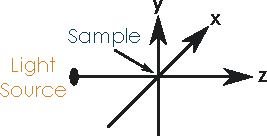
\includegraphics[width=0.6\textwidth]{figures/dx_CoordSystem.pdf}
\caption{The coordinate system used by CXI. The intersection of the X-ray beam with the sample define the  origin of the system. The z axis is parallel to the beam and points downstream.}
\label{fig:CoordSystem}
\end{figure}

\subsubsection{The local coordinate system of objects}
\label{OriginOfObjects}

For many detectors their location and orientation is crucial to interpret results.  Translations and rotations are used to define the absolute position of each object. But to be able to apply these transformations we need to know what is the origin of the local coordinate system of each object. Unless otherwise specified the origin should be assumed to be the geometrical center of the object in question. The default orientation of the object should have the longest axis of the object aligned with the x axis, the second longest with the y axis and the shortest with the z axis.


%****************************************************************************

\end{document}
